% !TeX root = main.tex
\documentclass[pdftex,
a4paper,
11pt,
parskip=half % Removes the horizontal indet when starting a new paragraph.
]{scrartcl}   
%
%---------------------------------------------------
%----- Packages
%---------------------------------------------------
%
\usepackage[T1]{fontenc}
\usepackage[utf8]{inputenc}
% This template is for english text only. You need to change it to German and adapt to your needs. We only provide English templates.
\usepackage[english]{babel}  
\usepackage{ae} 
\usepackage{fancyref} 
\usepackage{fancyhdr} % Define simple headings 
\usepackage{xcolor}
\usepackage{minted}
\usepackage{url}
\usepackage[pdftex]{graphicx}  
\usepackage{hyperref} % turn all your internal references into hyperlinks
\renewcommand{\sectionautorefname}{Section} %rename subsection to Section for better referencing
\renewcommand{\subsectionautorefname}{Section}
\renewcommand{\subsubsectionautorefname}{Section}

% ToDo List
\usepackage{enumitem,amssymb}
\newlist{todolist}{itemize}{2}
\setlist[todolist]{label=$\square$}
\usepackage{pifont}
\newcommand{\cmark}{\ding{51}}%
\newcommand{\xmark}{\ding{55}}%
\newcommand{\done}{\rlap{$\square$}{\raisebox{2pt}{\large\hspace{1pt}\cmark}}%
\hspace{-2.5pt}}
\newcommand{\wontfix}{\rlap{$\square$}{\large\hspace{1pt}\xmark}}

\definecolor{fu-orange}{RGB}{255,153,0}

% Fancy Tabellen
\usepackage{tabularx}
\definecolor{usethiscolorhere}{rgb}{0.92,0.92,0.92}
\definecolor{bamacolor}{RGB}{197, 210, 228}
\usepackage{booktabs}  
% own column Type Y!!!
\usepackage{ragged2e}  % for '\RaggedRight' macro (allows hyphenation)
\newcolumntype{Y}{>{\RaggedRight\arraybackslash}X}

% For the ganntchart
\usepackage{pgfgantt}
% a new command is defined that allows to include an empty page when needed

\usepackage{afterpage}


\newcommand{\blankpage}{
\newpage
\thispagestyle{empty}
\mbox{}
\newpage
}
%
%---------------------------------------------------
%----- PDF and document setup
%---------------------------------------------------
%
\hypersetup{
	pdftitle={<My title>},  % please, add the title of your thesis
    pdfauthor={<Author>},   % please, add your name
    pdfsubject={<<Bachelor thesis>, Institute of Computer Science, Freie Universität Berlin>}, % please, select the type of this document
    pdfstartview={FitH},    % fits the width of the page to the window
    pdfnewwindow=true, 		% links in new window
    colorlinks=false,  		% false: boxed links; true: colored links
    linkcolor=red,          % color of internal links
    citecolor=green,        % color of links to bibliography
    filecolor=magenta,      % color of file links
    urlcolor=cyan           % color of external links
}
%
%---------------------------------------------------      
%----- Settings for word separation  
%---------------------------------------------------      
% Help for separation (from package babel, section 22)):
% In german package the following hints are additionally available:
% "- = an explicit hyphen sign, allowing hyphenation in the rest of the word
% "| = disable ligature at this position. (e.g., Schaf"|fell)
% "~ = for a compound word mark without a breakpoint (e.g., bergauf und "~ab)
% "= = for a compound word mark with a breakpoint, allowing hyphenation in the composing words
% "" = like "-, but producing no hyphen sign (e.g., und/""oder)
%
% Describe separation hints here:
\hyphenation{
% Pro-to-koll-in-stan-zen
}

%---------------------------------------------------      
%----- Settings for title page 
%---------------------------------------------------

\begin{titlepage}

 
\title{
% TODO: Select the type of the thesis proposal you are writing.
% Source: https://degree.studentnews.eu/
{\normalsize --B. Sc. Thesis Proposal\footnote{Template Version 2.0 --- 2021-07-14}--\\
% TODO: The title should be capitalized. If unsure use the following website: https://capitalizemytitle.com/
[4ex]
{\LARGE Evaluation of requirements and implementation of a modern UI Editor}\\ 
[4ex]
\small Freie Universität Berlin\\Institute of Computer Science}\\
{\small Human-Centered Computing (HCC) Research Group}\\
[2ex]
}

\author{
% TODO: Add your full name here.
{\normalsize Matthias Kind}\\
% TODO: Add your matriculation number!
{\normalsize Student Number: 5338650}\\
% TODO Please use the email address provided by FU Berlin.
{\normalsize matthias.kind@fu-berlin.de}\\
% TODO: Add the date. This is important, since there will be different versions of you proposal.
{\normalsize Date of Proposal Submission: 2.11.2022}\\
% TODO: Please add the version, so we can keep track of the number of iterations.
{\normalsize Version: 2}\\
\rule{\textwidth}{0.4pt}\\
\\
{\normalsize Supervisor:}\\
% TODO: Add the name of your supervisor.
{\normalsize{Florian Berger\footnote{Department of Mathematics and Computer Science, Human-Centered Computing Research Group}, Freie Universität Berlin, Germany}}\\\\
{\normalsize Examiner:}\\
{\normalsize Prof. Dr. Claudia Müller-Birn\footnote{Department of Mathematics and Computer Science, Human-Centered Computing Research Group}, Freie Universität Berlin, Germany}\\
% TODO: Add the name of your second reviewer.
{\normalsize <Prof. Dr. Second Examiner\footnote{Department of Mathematics and Computer Science, <Name of Research Group>}>, Freie Universität Berlin, Germany}\\\\
} % end of \author

\date{} % This omits the date on the title page.

\end{titlepage}

%---------------------------------------------------      
%----- Setting up your document 
%---------------------------------------------------

\begin{document}

\maketitle
\thispagestyle{empty} % remove page number on the title page

%---------------------------------------------------
%----- GUIDELINES - Please remove this part before handing in your expose.
%---------------------------------------------------
% \pagecolor{fu-orange}

\section*{Guidelines}
\emph{Please remove this section before handing in your proposal.}

You should plan 3--4 feedback rounds for finalizing your proposal.
Before handing in the proposal to your supervisor, please check if your proposal fulfills the following criteria:

\begin{todolist}
  \item A proposal for a B. Sc. thesis should have about five pages of text. Excluding the title page, the timeline, references, and the outline.
  \item A proposal for an M. Sc. thesis should have a maximum of 10 to 20 pages. Please keep in mind, the text can be used for the thesis document. 
  \item Your proposal has to include a clearly stated research question. The research question has to be in the form of a sentence ending with a question mark.
  \item Include the assumed deadline for submitting your thesis in the timeline.
  \item Define a short, significant title that reflects the contents of your thesis. Please note, you can change the title in the final version.
  \item Use American English, for example, instead of vi\textbf{s}ualisation (BE) $\rightarrow$ visuali\textbf{z}ation (AE).
  \item You can write the proposal and also the final thesis either in German or in English. However, we recommend English. If you use German, please adapt the latex template on your own.
  \item The proposal should be comprehensible, so that not only specialists can understand it.
  \item Use correct spelling and grammar, as well as correct scientific language. Please use ''they'' as a gender neutral pronoun, rather than ''he or she,'' ''he/she,'' or ''s/he''. Using explicitly gendered pronouns excludes non-binary individuals and people who do not use solely binary ''he'' or ''she'' pronouns. For further information, please read Scheuerman et al.~\cite{scheuerman2020:hcigenderguidelines}.
  \item Use the ACM citation style.
  \item Avoid any indication of possible plagiarism. Please remember, in severe cases, plagiarism results in a fail.
 
\end{todolist}

\subsection*{Where to find literature?}
Be aware that the Human-Centered Computing (HCC) Research Group conducts research in the areas of Human-Computer Interaction (HCI) and Collaborative Computing. Therefore, articles from the following conferences are of particular interest\footnote{Upcoming conference are listed on the website of the ACM Special Interest Group on Computer-Human Interaction (CHI): \url{https://sigchi.org/conferences/upcoming-conferences/}}: 

\begin{itemize}
    \itemsep0em % This should move to the global layout section.
    \item CHI --- Human Factors in Computing Systems
    \item CSCW --- Computer Supported Cooperative Work
    \item IUI --- International Conference on Intelligent User Interfaces
    \item DIS --- Designing Interactive Systems Conference
\end{itemize}

You can find the publications of these conferences in the Digital Library of ACM\footnote{ \url{https://dl.acm.org/}}. We highly recommend this search engine, as opposed to using the general search engine Google Scholar\footnote{\url{https://scholar.google.com/}}. In ACM, the papers are already contextualized (by considering the respective conference in the search filters), and thus, you ensure that the work is relevant. If you have any doubts, talk to your supervisor.

\subsection*{What is a human-centered design approach?}
At HCC Research Group, we always apply a human-centered design (HCD) approach. This approach is taught in the \emph{Human-Computer Interaction I} course. If you are not familiar with this approach, you need to learn it before starting your thesis. Please contact your supervisor to get access to the slides and videos of the course. In order to reach your goals, you have to make sure that you understand which research methods are most suitable to fulfill your goals. We recommend reviewing available methods and their practical application in the field of HCI~\cite{lazar2017research, olson2014ways}. Both mentioned sources and additional books are available at the HCC Research Group's library\footnote{We also set up an open Zotero library where we share literature references that have shown to be helpful in prior theses regarding fundamental knowledge on HCI methods. You can find the open Zotero library ''HCC --- Thesis Literature'' here: \url{https://www.zotero.org/groups/2815440/hcc_-_thesis_literature}.}. Please talk to your supervisor.


\afterpage{\nopagecolor}

%---------------------------------------------------
%----- Summary
%---------------------------------------------------
% !TeX root = main.tex
\section*{Summary}
The goal of the proposed thesis is to conceptualize and develop an UI Editor to create and configure Apps and Web-Apps for digital publishers. These Apps are based on an existing domain specific web framework, developed by \url{https://sprylab.com}. Apps are configured via dynamic resources, which contain all the styles, scripts and configs needed to render the customer's app on client devices.
To enable the targeted user groups like internal developers,
customer support and the customers (news and magazine publishers) to work more productive,
I want to collect their current painponts and ideas for improvement through various HCI methods and develop a new web-app to fulfill their requirements better.

As a baseline, this means a fast and easy to use interface which prevents user errors from happening or gives feedback on their actions, while also giving more advanced users the abilities they need to do their changes. The editor to configure the Apps UI should be proceduraly generated from the source files of the framework and be performant enough to handle large configurations.


%---------------------------------------------------
%----- Contents
%---------------------------------------------------
\tableofcontents

 % page number is set to "1" otherwise it would be "3"
\setcounter{page}{1}

%---------------------------------------------------      
%----- CONTENT PART 
%---------------------------------------------------
%---------------------------------------------------
%----- Introduction
%---------------------------------------------------
% !TeX root = main.tex
%************************************************************************
\section{Introduction}
\label{sec:introduction}
% Introduction to the topic.
% Explain why this work is important giving a general introduction to the subject,
% list the basic knowledge needed and outline the purpose of the report. 
%************************************************************************
The company Sprylab provides an software platform to publishers to provide their print- and digital content to their users. The user-facing part of that platform is an web framework based on Angular, which is rendered in Apps or as a Website and provides the customers components and data sources usually required by apps in this domain.

The app specific data is stored on "dynamic resources", which utilize a specific folder structure and contain common files used by web-apps, like static images, CSS and Javascript files, and the configuration files that declare the UI rendered by the app.

%************************************************************************
\subsection{Motivation}
\label{subsec:motivation}
% Motivation and relevance of the topic.
%************************************************************************
Editing these dynamic resources by hand is tedious and error-prone, as the manual workflow consists of downloading a ZIP file, editing the contents and uploading without any validation before the resources are deployed to the app.

This requires a deep knowledge of the setup, what files and keys to put where, and still experienced users of the framework can easily introduce errors by misspelling a filename or putting a wrong component name inside the UI declaration files.

An existing attempt to have a web-based editor were not pursued with much ambition or proper requirements analysis to provide a pleasant user experience to users besides the original framework developers.
Thus, current ''non-power-users'' often struggle with slow performance, missing explainations or cryptic error messages.

Besides the often unpleasant user experience, it also suffered from bad developer experience, like non-optimal project setups and the limits of existing libraries that were used,
e.g. to edit the UI declarations based on specific schemata.

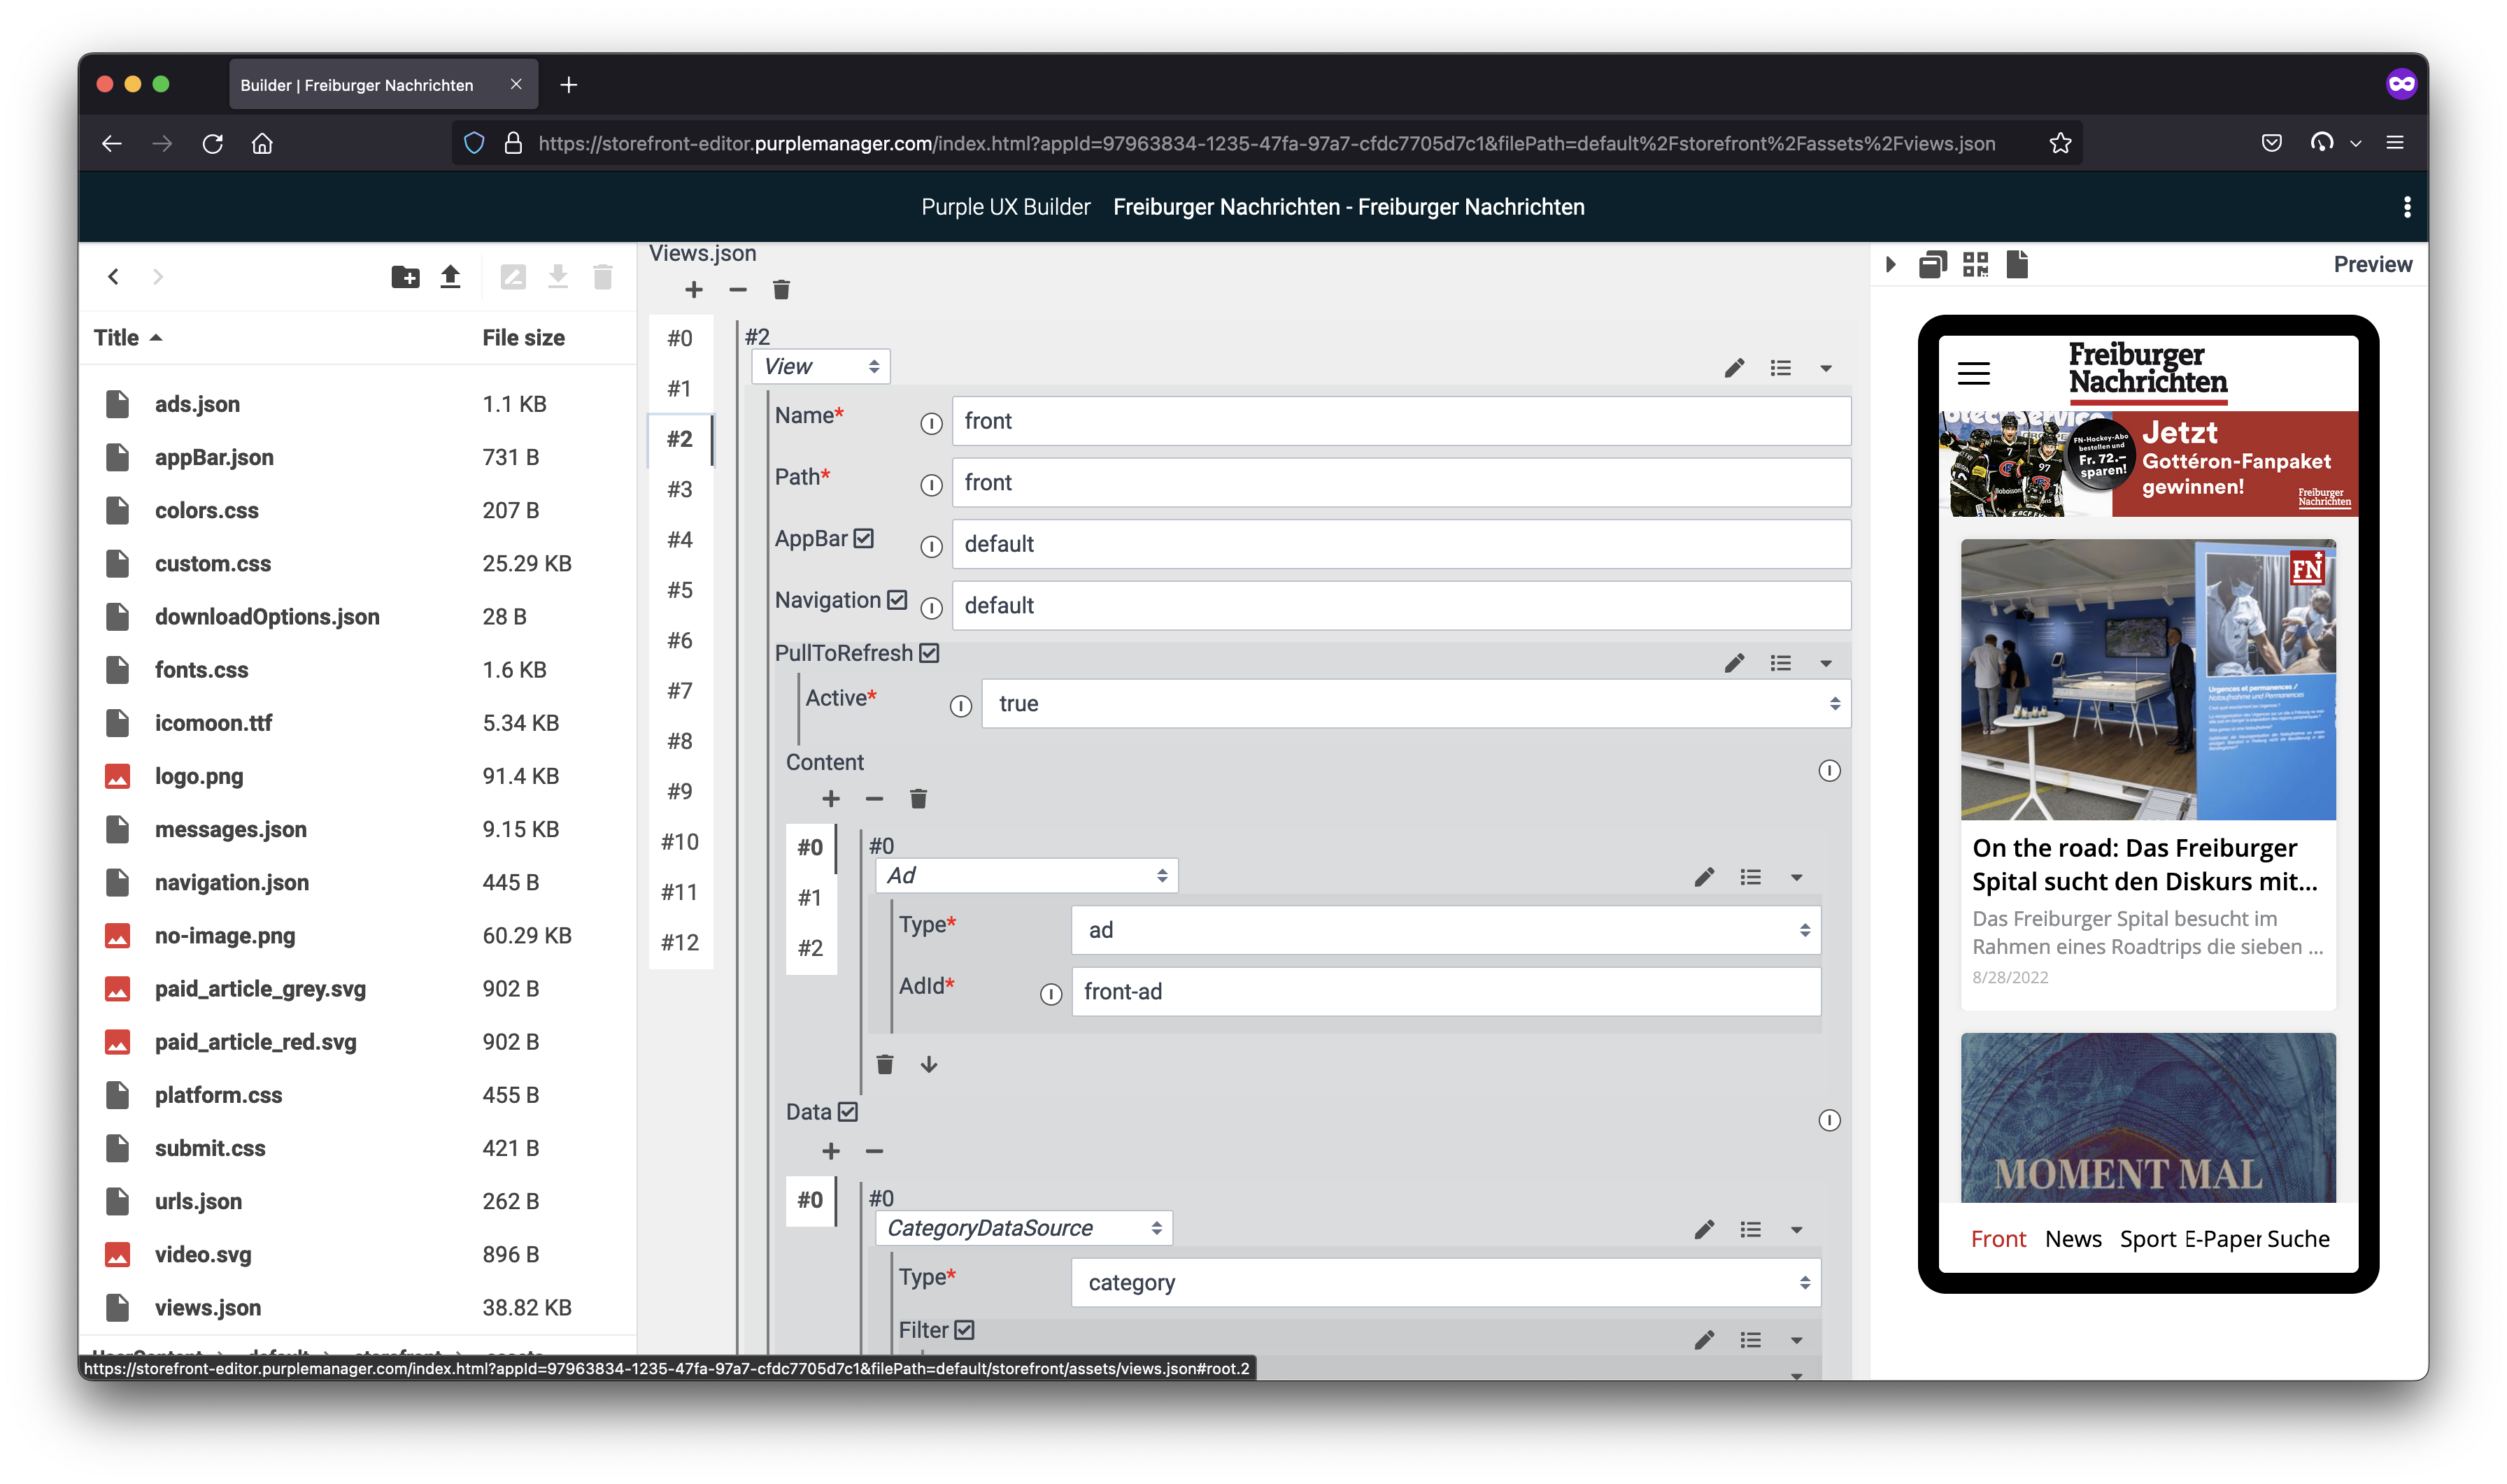
\includegraphics[width=\textwidth]{pics/current_editor.png}
An example of the current editor UI

%************************************************************************
\subsection{Goal}
\label{subsec:goal}
% Gap you want to close with your research.
% Goal of your work.
% Your research question.
% List the main research question(s) you want to answer.
% Explain whether your research will provide a definitive answer or simply contribute towards an answer
%************************************************************************
The goal is to give the diffrent identified possible user groups an editor
which enables them to work more productive, make less errors and get more interactive feedback from the system,
so that there is less support needed by other entities like the framework developers.


This includes evaluating diffrent HCI methods to evaluate the current state as well as the diffrent needs of the users,
and then using an agile development process to build an web based editor for the Purple Experience framework.
The core of this will be an editor to edit the JSON files describing the App's UI, respecting JSON schema definitions
and fitting the users diffrent knowledge and skill levels.

On a more abstract level, the outcome of the thesis should give insights about integrating an new tool / UI into an existing
production enviroment with many constraints, which methods and approaches worked and maybe also which failed.

The contributions I aim to produce with this bachelor thesis are:

\begin{description}[leftmargin=10em,style=nextline]
  \item[software] an web app and backend that serves and present the editor to clients, possibly contributions to open source libraries if required to fulfill the needs of the editor.
  \item[HCI discoveries] documentation to the diffrent methods and approaches used to gain the insight into the users,
  as well as evaluation of the results of these methods and how effective they proved in the context of changing a component inside a larger ecosystem.
  \item[user base knowledge] better knowledge about what the diffrent user groups of the propsed editor are and can be, as well as their diffrent habits, knowledge levels, common mistakes and more.
\end{description}


%---------------------------------------------------
%----- Background
%---------------------------------------------------
% !TeX root = main.tex
%************************************************************************
\section{Background}
\label{sec:background}
% List relevant work by others,
% or preliminary results you have achieved with a detailed and accurate
% explanation and interpretation.
% Include relevant photographs, figures or tables to illustrate the text.
% This section should frame the research questions that your subsequent research will address. 
%************************************************************************
Please add a sentence that summarizes what this section is about and what the reader can expect.
%************************************************************************
\subsection{Context of the Project and Problem Description} 
\label{sec:context}
%************************************************************************
Explain all the surroundings that are necessary to understand the broader context of your work. If necessary, give a brief introduction to non-HCI research literature as background knowledge. It is best to include a specific scenario\footnote{Scenarios are defined as an \emph{''informal narrative description''}. \emph{''It describes human activities or tasks in a story that allows exploration and discussion of contexts, needs, and requirements. It does not necessarily describe the use of software or other technological support used to achieve a goal. Using the vocabulary and phrasing of users means that scenarios can be understood by stakeholders, and they are able to participate fully in development.''}~\cite{preeceInteractionDesignHumancomputer2015}.}. If you are designing a piece of software or graphical user interface, please specify your users and the tasks the users want to perform with your software.

%************************************************************************
\subsection{Related Work}
\label{sec:relatedwork}
%************************************************************************
This section consists of a literature review to situate your thesis in the scientific context. Which academic articles exist in your problem area, and how are they related to your work? When placing your thesis in the context of others, you need to consider other work, which uses a similar methodology or articles, who try to answer similar research questions.

\begin{table}[htb]
\small
\colorbox{bamacolor}{
\centering
\begin{tabularx}{\textwidth}{@{} r Y @{}}
	&
	\textbf{Distinction between Bachelor and Master thesis}\vspace{2mm}\\
    \textbf{B. Sc. Thesis} &
    A small literature review is mandatory, starting with the articles your supervisor provides. The related work part can also include a mini similar tool analysis if you are implementing a specific part of a software. \vspace{2mm}\\
	\textbf{M. Sc. Thesis} &
	A literature review is mandatory. If it is part of your project to choose a specific framework, then you need to conduct a short survey on existing frameworks. This also applies if you want to choose an algorithm to perform a specific task or want to design a study. \vspace{2mm}\\

\end{tabularx}
}
\end{table}

In the thesis announcement\footnote{Thesis announcements are descriptions for ''Open Theses'' on the HCC website: \url{https://www.mi.fu-berlin.de/en/inf/groups/hcc/theses/open/index.html}} already, relevant literature is provided. If this is not the case, please ask your supervisor for articles. Describing the state of the art is essential to identify the gap you would like to fill. Thus, the literature's description should clearly result in research gaps that lead to specific research questions. 


%************************************************************************
\subsection{Research Questions}
\label{subsec:question}
% Based on your overarching goal and the reviewed research, specify your research question.
%************************************************************************
In this section, you should name your research questions. Your research question should be based on the observation that prior research has a gap and some misconception. You can use words such as \emph{but} or \emph{however} to indicate this. Make sure that your emphasize the significance of your research. 
%---------------------------------------------------
%----- Your methodology approach
%---------------------------------------------------
%************************************************************************
\section{Methodology}
\label{subsec:methodology}
% Explain the methods and techniques which will be used for your project depending on the subject: field work, laboratory work, modeling technique, interdisciplinary collaboration, data type, data acquisition, infrastructure, software, etc.
%************************************************************************
Specify the overall methodology you want to apply in order to reach your goals and answer your research questions. We often apply the HCD process (cf.~\autoref{fig:hcd}): 1. Vision, 2. Analyze, 3. Design for Usability, 4. Construct and Deploy (Implementation), 5. Evaluate in Context, 6. Feedback. There is no predefined ready-to-use HCD process. You need to adapt the general process presented to your project. This means you need to think of specific methods in each step of the process. Please link your planned procedure to your goals. If your thesis follows a data science workflow, please adapt your methodology accordingly. It is not necessary to go through all the phases of the design process in detail, it is also possible to limit the number of iterations or focus on one particular phase. This depends on your project.

This chapter explains what method was chosen in the HCD process and why it helps to answer your research question.
\\
\hrule

Ref: ''Learn Human computer interaction'', 104 diagram

\subsection{Analyze}
\label{subsec:analyze}

\textbf{1st phase ''discovery'':} assess currecnt situation through various User Research methods (taken from ''Learn Human computer interaction'', 132: Human Centered Methods for User Research)

\begin{itemize}
  \setlength\itemsep{-0.2em}
  \item fly-on-the-wall method: observe without users knowing they are observed
  \item moderated observation: Create scenario for user and note the way(s) the users do the task
  \item user interviews: prepare questions on workflows, what they are missing, what takes most time
  \item Quantitative survey
\end{itemize}


\subsection{Design for Usability and early prototyping}
\label{subsec:design}

Build deployable prototype using agile development methods

\begin{itemize}
  \setlength\itemsep{-0.2em}
  \item Evaluate methods from 1st phase on effectiveness and continue using them with test circle of persons
  \item Use SCRUM to plan work
  \item use CI/CD to allow fast iterations after changed requirements
  \item Build in Analytics / Tracking service for automatic user data evaluation
  \item A/B testing?
\end{itemize}


\subsection{Construct (Implementation)}
\label{subsec:implementation}

This section is closely coupled to \ref{subsec:design}, this construction of the software results from the prototypes and is done in the same SCRUM sprints as the design.

The tech stack is one of the constraints imposed by the environment,
the backend will be written in Javascript for NodeJS \and express as the web framework.

The frontend, including the JSON editor should be written in react to utilize exisitng knowledge from other developers at the company and to guarantee long support.
The backend will be hosted as a docker container on a kubernetes cluster and easily deployable via gitlab Continous integration systems.

Depending on the collected requirements during the first phase, we might also integrate REDIS as a light messanging bus to support multiple instances.\\

\begin{figure}[h]
  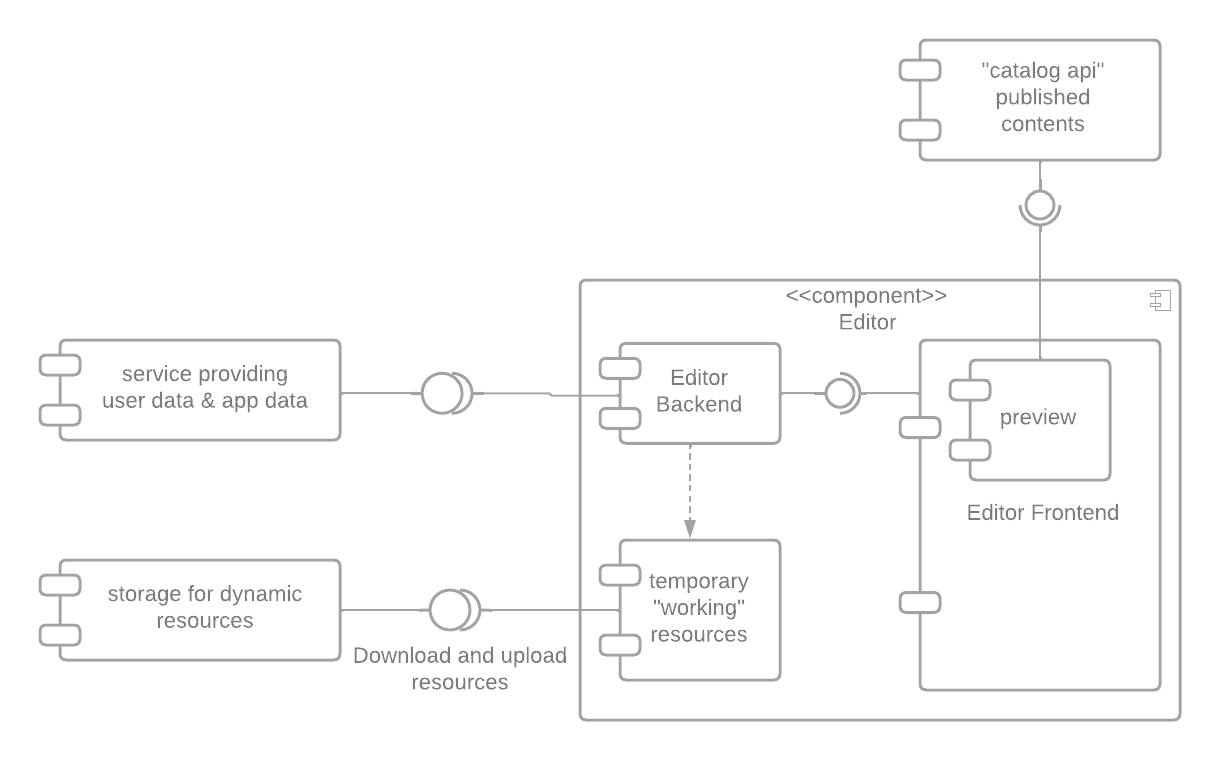
\includegraphics[width=0.7\textwidth]{pics/editor_uml_component.png}
  \caption[]{UML component diagram of the integration into the exisitng environment}
\end{figure}



\subsection{Evaluation}
\label{subsec:evaluation}

The evaluation towards the end of the thesis consists of using some of the methods mentioned above a last time. There the focus will probably be on a survey and evaluating analytics data, as well as getting verbal feedback from test users.
The results then get compared to the results raised earlier to identify improvements in the productivity of the users.

From that results, more abstract realizations about developing new software with HCI methods in constrained exisitng environments can be elaborated.

%---------------------------------------------------
%----- Preliminary schedule and planned milestones
%---------------------------------------------------
\section{Project Plan}
\label{sec:plan}

It is useful to understand a Bachelor and Master thesis as a project. Projects are based on a plan, and each plan needs milestones\footnote{By milestone we mean a collection of tasks, which need to be finished by a specific date. You can also call it a work package.} and a timeline. Thus, in this section, you will break down your thesis project into manageable and specific milestones to realistically estimate the time you need. Especially if you use methods for the first time, we recommend to discuss this timeline with your supervisor. Please describe each milestone, what do you exactly do in that phase, in what order, what is the result or outcome of each step, and how does it contribute towards the goal of your thesis. As a result, you will outline a detailed timeline for your upcoming research.

According to the exam regulations: a Bachelor thesis\footnote{Please read \S~10 of the Study and Examination regulations for the bachelor’s degree program: \url{https://www.imp.fu-berlin.de/fbv/pruefungsbuero/Studien--und-Pruefungsordnungen/StOPO_BSc_Inf_-2014.pdf}, accessed May 16, 2021} takes about 360~hours (12~LP) and a Master thesis\footnote{Please read \S~9 of the Study and Examination regulations for the master’s
degree program: \url{https://www.imp.fu-berlin.de/fbv/pruefungsbuero/Studien--und-Pruefungsordnungen/STOPO_MSc_-Inf_-2014.pdf}, accessed May 16, 2021} is calculated with 900~hours (30~LP).

\begin{table}[htbp]
\small
\colorbox{usethiscolorhere}{
\centering
\begin{tabularx}{\textwidth}{@{} r Y @{}}
	& \begin{todolist}
  \itemsep0em % This should move to the global layout section.
  \item Calculate the hours you can effectively work on your thesis per week.
  \item Write down the planned date of handing in your thesis.
  \item Include up to 40~\% buffer in case of unforeseen problems (e.g., sickness, vacation).
  \item Include a Gantt-Chart.
\end{todolist}\\
    
\end{tabularx}
}
\end{table}




\subsection{Milestones}
\label{subsec:milestone}
Specify the milestones of your upcoming project. Please describe when you plan to achieve which milestone and what artifact(s) or outcome will result from each milestone. Also, keep in mind what the goal of each milestone is.


\begin{table}[htbp]
\small
\colorbox{usethiscolorhere}{
\centering
\begin{tabularx}{\textwidth}{@{} r Y @{}}
	\textbf{M1}
	& \textbf{Milestone --- Literature Review}\vspace{2mm}\\
	\textbf{Due date} & 2021-05-26 (Week $2$)\vspace{2mm}\\
     \textbf{Tasks} & Identifying and read other studies/thesis/papers evaluating the usability of chatbots in a medical context\vspace{2mm}\\
    \textbf{Outcome} & A list of relevant papers (e.g. folder in Zotero).\\
    & A written summary for each paper.\\
    & A final text summarizing the main findings and approaches, which might be useful for my project. \vspace{2mm}\\
    \textbf{Goal} & General understanding of methods to evaluate the usability of chatbots in the medical context. Having a good foundation for discussing my results in the context of other people's work.\vspace{2mm}\\
    
\end{tabularx}
}
\end{table}

\begin{table}[htbp]
\small
\colorbox{usethiscolorhere}{
\centering
\begin{tabularx}{\textwidth}{@{} r Y @{}}
	\textbf{M2}
	& \textbf{Milestone --- Evaluate Wikipedia's Advanced Search Interface}\vspace{2mm}\\
	Due date & 2021-06-15 (Week $4$)\vspace{2mm}\\
     Tasks & Prepare, conduct, and evaluate a remote usability test with four participants.\vspace{2mm}\\
    Outcome & Moderator script for conducting the usability test.\\
    & Affinity diagram with thematic clusters and headlines.\\
    & A list of usability issues sorted by severity.\vspace{2mm}\\
    Goal & Understanding the drawbacks of the current Wikipedia advanced search in order to (re)design a new interface.\vspace{2mm}\\
    
\end{tabularx}
}
\end{table}

\begin{table}[htbp]
\small
\colorbox{usethiscolorhere}{
\centering
\begin{tabularx}{\textwidth}{@{} r Y @{}}
	\textbf{M...}
	& \textbf{Milestone ---  ...}\vspace{2mm}\\
    Due date & \mbox{} \vspace{2mm}\\
    Tasks & \mbox{} \vspace{2mm}\\
    Outcome & \mbox{} \vspace{2mm}\\
    Goal & \mbox{} \vspace{2mm}\\
\end{tabularx}
}
\end{table}

\begin{table}[htbp]
\small
\colorbox{usethiscolorhere}{
\centering
\begin{tabularx}{\textwidth}{@{} r Y @{}}
	\textbf{M5}
	& \textbf{Milestone ---  High-Fidelity Prototype}\vspace{2mm}\\
	Due date & 2021-08-15 (Week $15$)\vspace{2mm}\\
     Tasks & Implement the final design and the main features with HTML and CSS. \vspace{2mm}\\
    Outcome & Repository with code and data on GitLab.\\
    & Deployed on Heroy and public link.\vspace{2mm}\\
    Goal & Interactive prototype, which is deployed and ready for testing.\vspace{2mm}\\
\end{tabularx}
}
\end{table}

\clearpage
\subsection{Timeline}
\label{subsec:timeline}
Now you need to transfer the milestones into a timeline. The time for your thesis will help you to set realistic time goals and maybe reconsider milestones. Use a Gantt chart\footnote{Check out Wikipedia for an extended overview of project management software that fits your needs: \url{https://en.wikipedia.org/wiki/Comparison_of_project_management_software}. For example Ganttproject is free of charge and open source: \url{https://www.ganttproject.biz/}, accessed: May 26, 2021} for visualization. Please consider what tasks you can do in parallel. Also indicate how you will handle the writing process within your timeline.

    \ganttset{%
        calendar week text={%
            \currentweek
        }%
    }

\begin{ganttchart}[
    hgrid, vgrid, bar label font=\small,
    x unit=1.5mm,
    time slot format=little-endian]{24-5-2021}{15-8-2021}
\gantttitlecalendar{ month=shortname, week=1} \\
    \ganttbar{M1}{24-05-2021}{6-06-2021}\\
    \ganttbar{M2}{7-06-2021}{20-06-2021}\\
    \ganttmilestone{Presentation}{20-06-2021} \\
    \ganttbar{M3}{15-06-2021}{5-7-2021}
    \ganttmilestone{}{5-07-2021} \\
    \ganttbar{Writing}{6-6-2021}{8-6-2021}
    \ganttbar{}{12-7-2021}{27-7-2021}\\
    \ganttbar{Correcting}{1-08-2021}{6-08-2021}
    \ganttmilestone{}{6-08-2021} \\
    \ganttbar{Buffer}{7-08-2021}{14-08-2021} \\
    \ganttmilestone{Submission}{15-08-2021}
\end{ganttchart}
%---------------------------------------------------
%----- Outline of your planned thesis
%---------------------------------------------------
\section{Preliminary Outline}
\label{sec:outline}
% The theoretical background should consist of definitions of significant concepts and terms and introduces your methods, approaches, and theories. The Discussion Section must include a reflection on your main results in the light of related work and your research goal and questions.

\small
\colorbox{usethiscolorhere}{
\centering
\begin{tabularx}{\textwidth}{@{} r Y @{}}
	\textbf{1}
	& \textbf{Introduction}\vspace{2mm}\\
	& 1.1 Motivation \vspace{2mm}\\
	& 1.2 Research goal and question\vspace{2mm}\\
	& 1.3 Research approach and methodology\vspace{2mm}\\
	\textbf{2}
	& \textbf{Theoretical Background}\vspace{2mm}\\
	& 2.1 Concepts and definitions of the Purple apps and the web framework \vspace{2mm}\\
	& 2.2 Introduction to the used HCI User Research methods \vspace{2mm}\\
	& 2.3 Introduction to the development process \vspace{2mm}\\
	\textbf{3}
	& \textbf{Related Work}\vspace{2mm}\\
    & 3.1 Related software\vspace{2mm}\\
    & 3.2 Related studies in this field\vspace{2mm}\\
	\textbf{4}
	& \textbf{Analysis}\vspace{2mm}\\
    & 4.1 Defining and conducting initial User Research\vspace{2mm}\\
    & 4.2 Collecting the structural requirements implied by the ecosystem\vspace{2mm}\\
    & 4.3 Derive requirements\vspace{2mm}\\
	\textbf{5}
	& \textbf{Design Process}\vspace{2mm}\\
    & 5.1 high- and low-fidelity prototyping\vspace{2mm}\\
	\textbf{6}
	& \textbf{Implementation}\vspace{2mm}\\
    & 6.1 Overview of system architecture\vspace{2mm}\\
    & 6.2 Technical implementation\vspace{2mm}\\
    & 6.3 Implementation of generative UI editor respecting JSON schemata\vspace{2mm}\\
    & 6.4 Using iterative development process methods in practice\vspace{2mm}\\
	\textbf{7}
	& \textbf{Evaluation}\vspace{2mm}\\
    & 7.1 present final conducted User Research methods\vspace{2mm}\\
    & 7.2 Present study results in comparison to inital state of the editing process\vspace{2mm}\\
    & 7.3 Evaluate study results regarding the thesis research question\vspace{2mm}\\
	\textbf{8}
	& \textbf{Discussion}\vspace{2mm}\\
	\textbf{9}
	& \textbf{Conclusion}\vspace{2mm}\\
    & 9.1 Limitations\vspace{2mm}\\
    & 9.2 Future Work\vspace{2mm}\\
\end{tabularx}
}
%---------------------------------------------------
%----- Bibliography
%---------------------------------------------------
\addcontentsline{toc}{section}{Bibliography}
\bibliographystyle{abbrv}  % citation style
\bibliography{references} % bib file
\end{document}